\chapter{Paketeinteilung}
\label{ch:paketeinteilung}

Die Paketeinteilung der Software gliedert sich in folgende Pakete: %TODO Paketübersicht

\section{graphmodel}

\begin{figure}[hb]
  \centering
  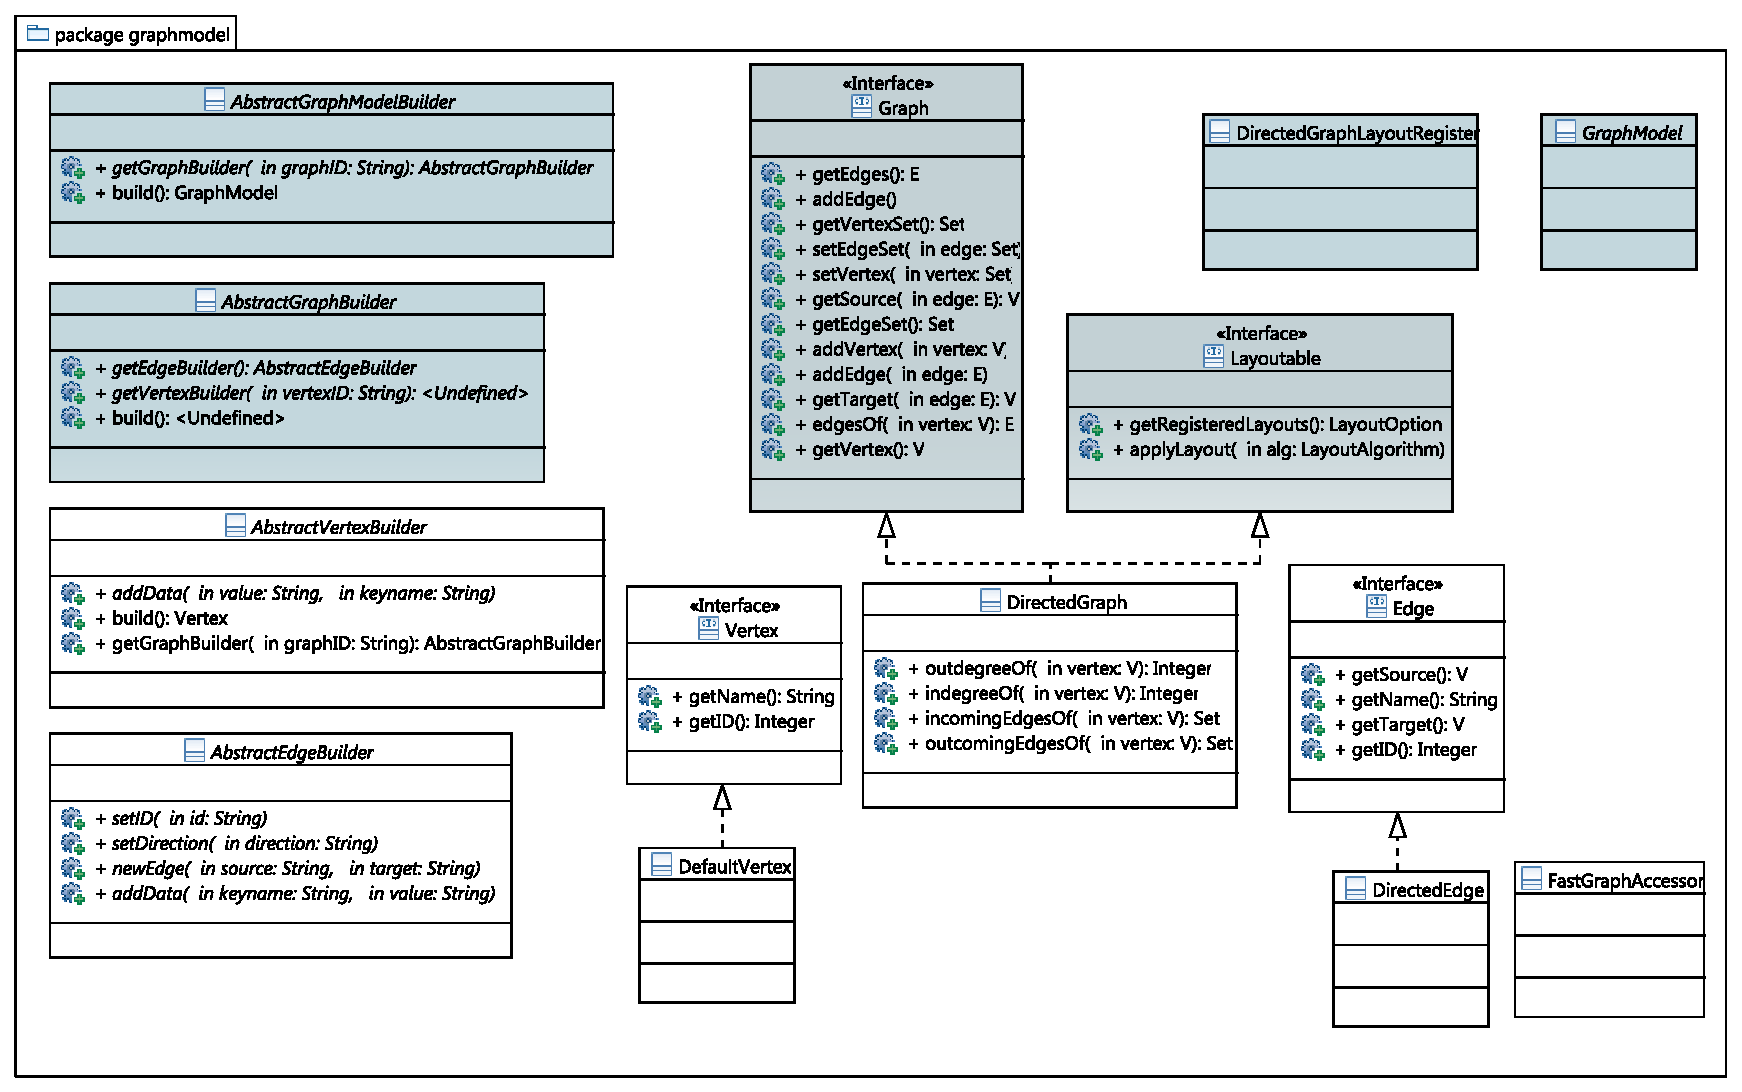
\includegraphics[width=380pt]{resourcen/graphmodel.pdf}
  \caption{Paketübersicht graphmodel}
  \label{fig:packge_graphmodel}
\end{figure}

In dem Paket graphmodel befinden sich die Klassen die für die interne Repräsentation des Graphen benötigt werden. Die Funktionalität dieses Pakets ist es ein flexibles Graph model sowie schnellen Zugriff auf dessen Komponenten bereitzustellen. Hierfür werden Interfaces für Graphen, Vertices und Edges bereitgestellt und teilweise schon implementiert. 

\newpage

\section{gui}

\begin{figure}[hb]
  \centering
  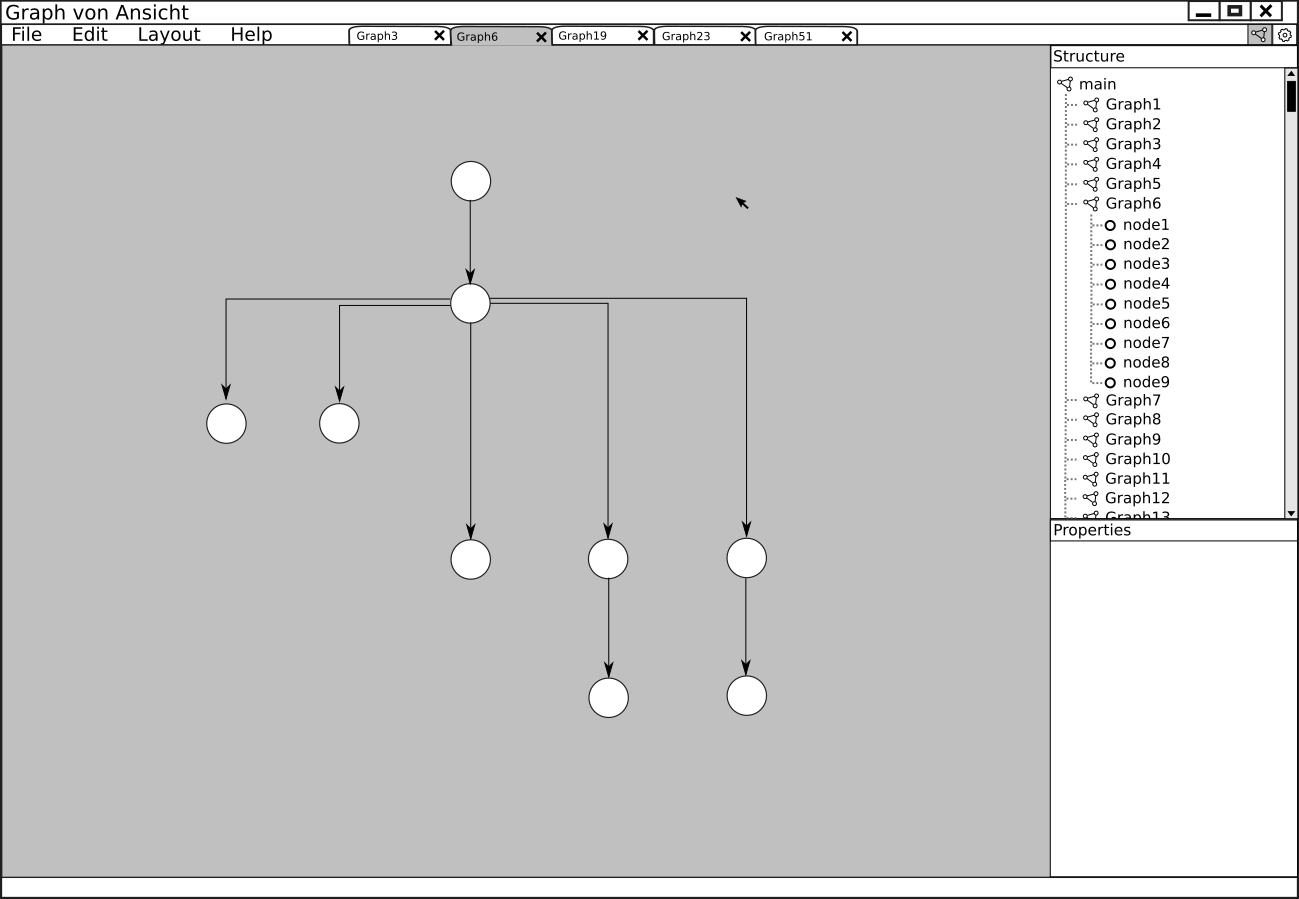
\includegraphics[width=380pt]{resourcen/gui.pdf}
  \caption{Paketübersicht gui}
  \label{fig:packge_gui}
\end{figure}

Das Paket gui beinhaltet die Anzeigenlogik. Hier werden Views und Elemente definiert die für die Anzeige notwendig sind. Dafür erweitern sie JavaFX Komponenten.

\newpage

\section{parameter}

\begin{figure}[hb]
  \centering
  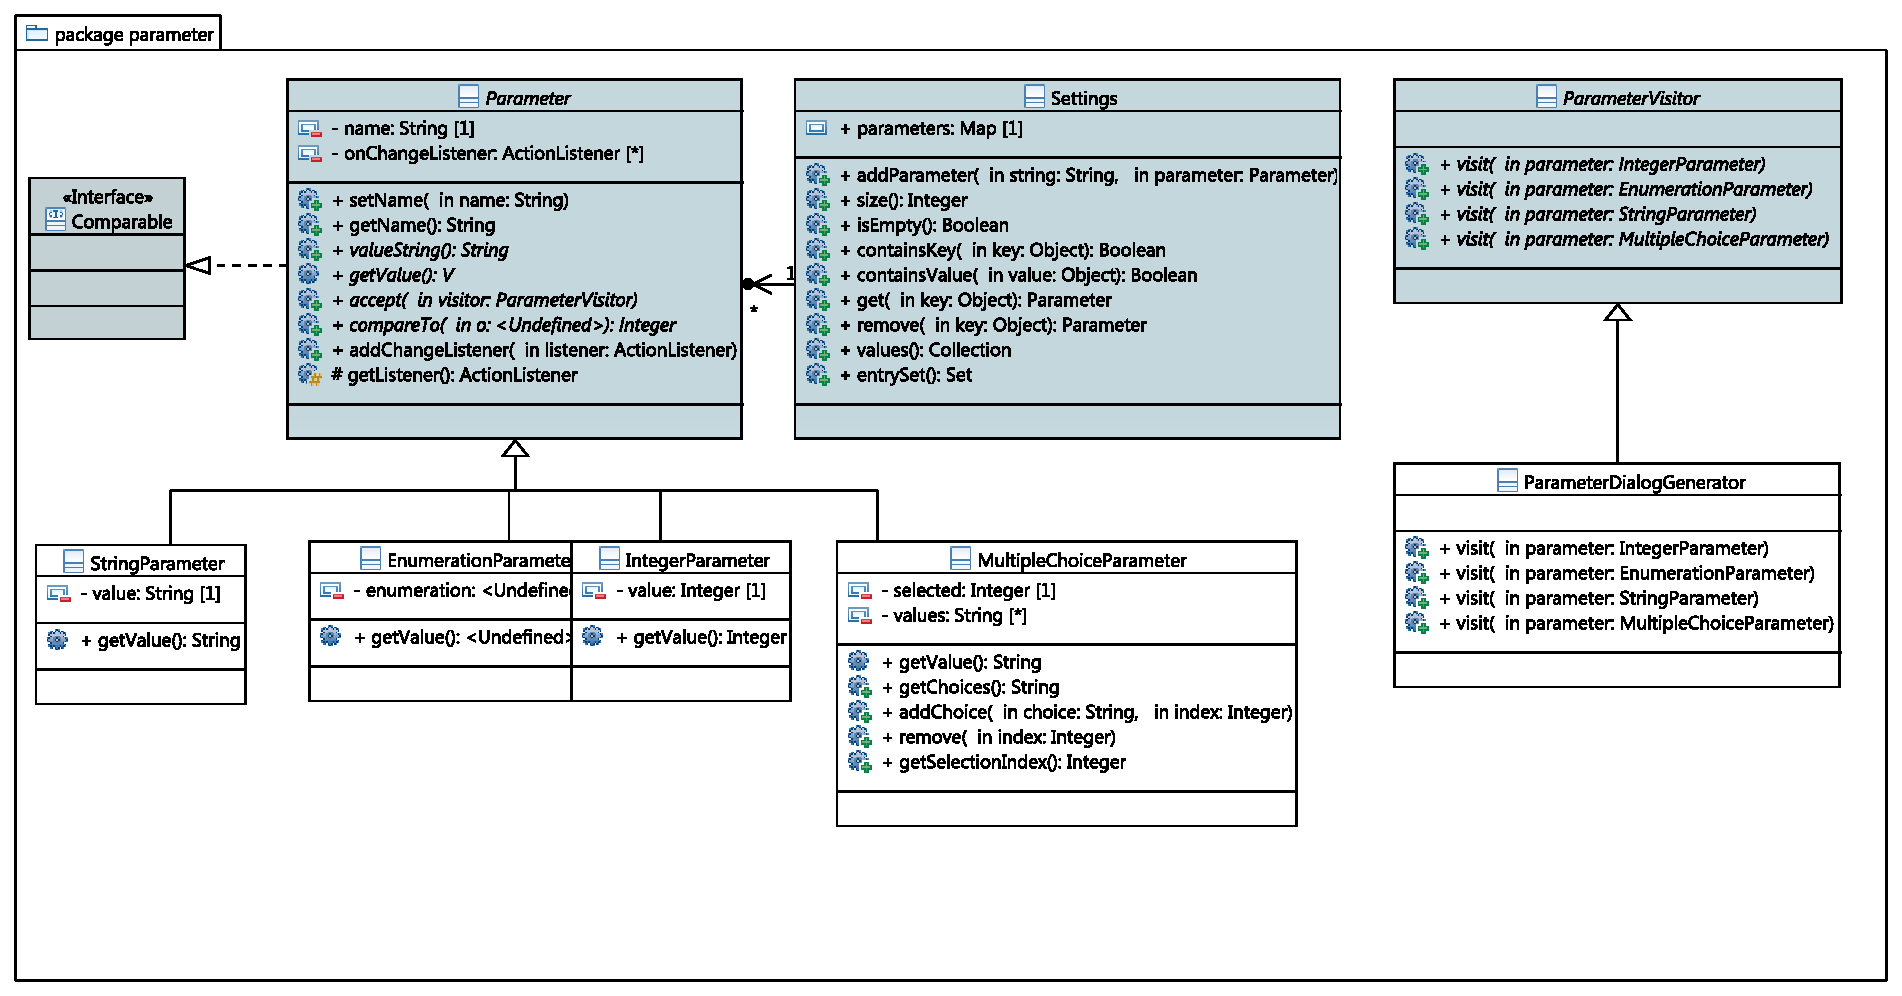
\includegraphics[width=380pt]{resourcen/parameter.pdf}
  \caption{Paketübersicht parameter}
  \label{fig:packge_parameter}
\end{figure}

Diese Paket trennt parameter vom Rest. Diese speziellen Wrapper erlauben dem plugins ihre Einstellungen an den View zu übergeben. Das selbe gilt auch für Constraints. Diese Wrapper Klassen beinhalten Methoden zur Umwandlung der jeweiligen Parameter in Zeichenketten aber auch vergleiche zum sortieren der Werte.

\newpage

\section{graphRegex}

\begin{figure}[hb]
  \centering
  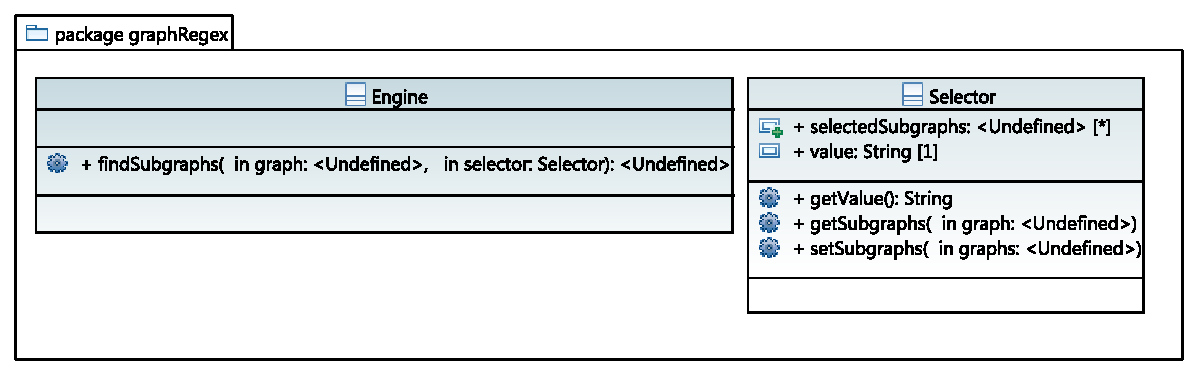
\includegraphics[width=380pt]{resourcen/graphRegex.pdf}
  \caption{Paketübersicht graphRegex}
  \label{fig:packge_graphRegex}
\end{figure}

In diesem Paket befinden sich die Algorithmen zum durchsuchen von Graphen nach Subgraphen mithilfe von Selektoren

\newpage

\section{objectpropert}

\begin{figure}[hb]
  \centering
  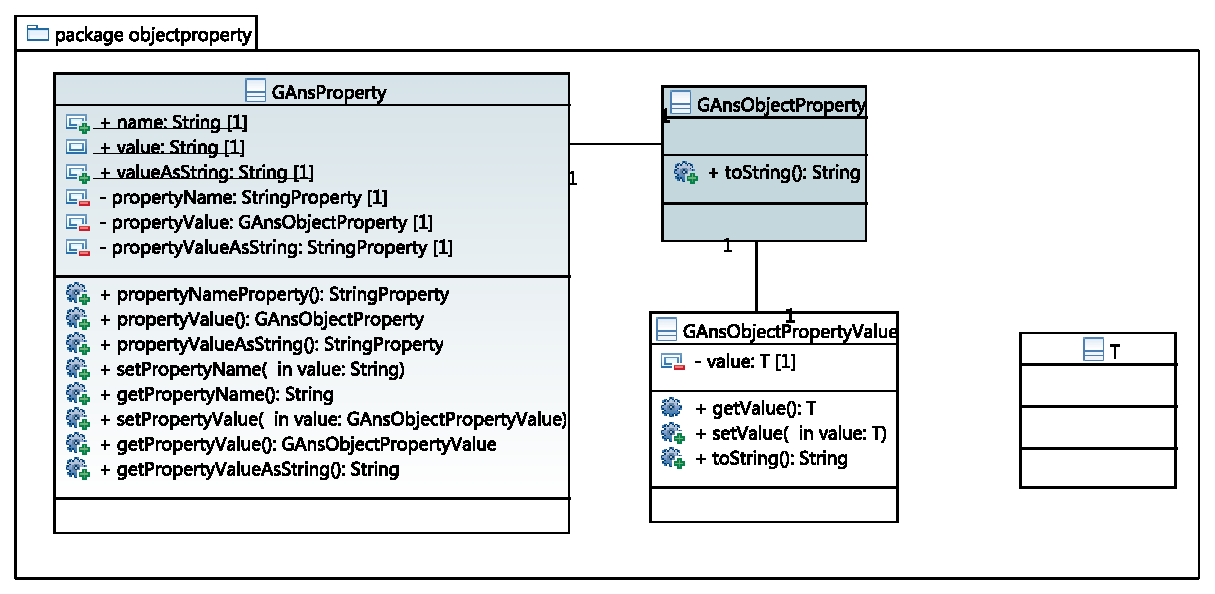
\includegraphics[width=380pt]{resourcen/objectproperty.pdf}
  \caption{Paketübersicht objectproperty}
  \label{fig:packge_objectproperty}
\end{figure}

\newpage

\section{plugin}

\begin{figure}[hb]
  \centering
  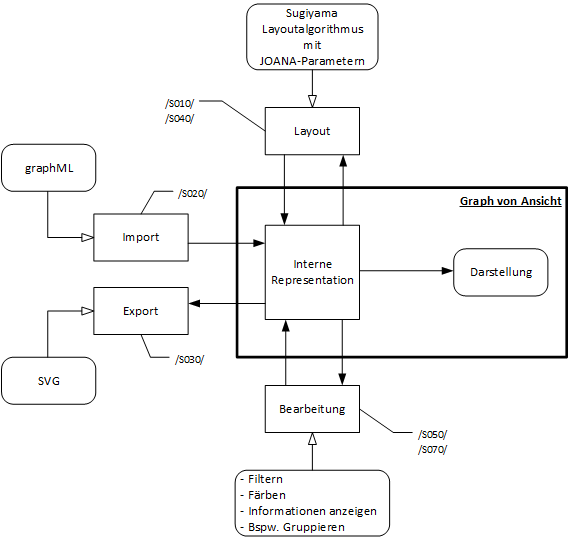
\includegraphics[width=380pt]{resourcen/plugin.pdf}
  \caption{Paketübersicht plugin}
  \label{fig:packge_plugin}
\end{figure}

\newpage

\section{sugiyama}

\begin{figure}[hb]
  \centering
  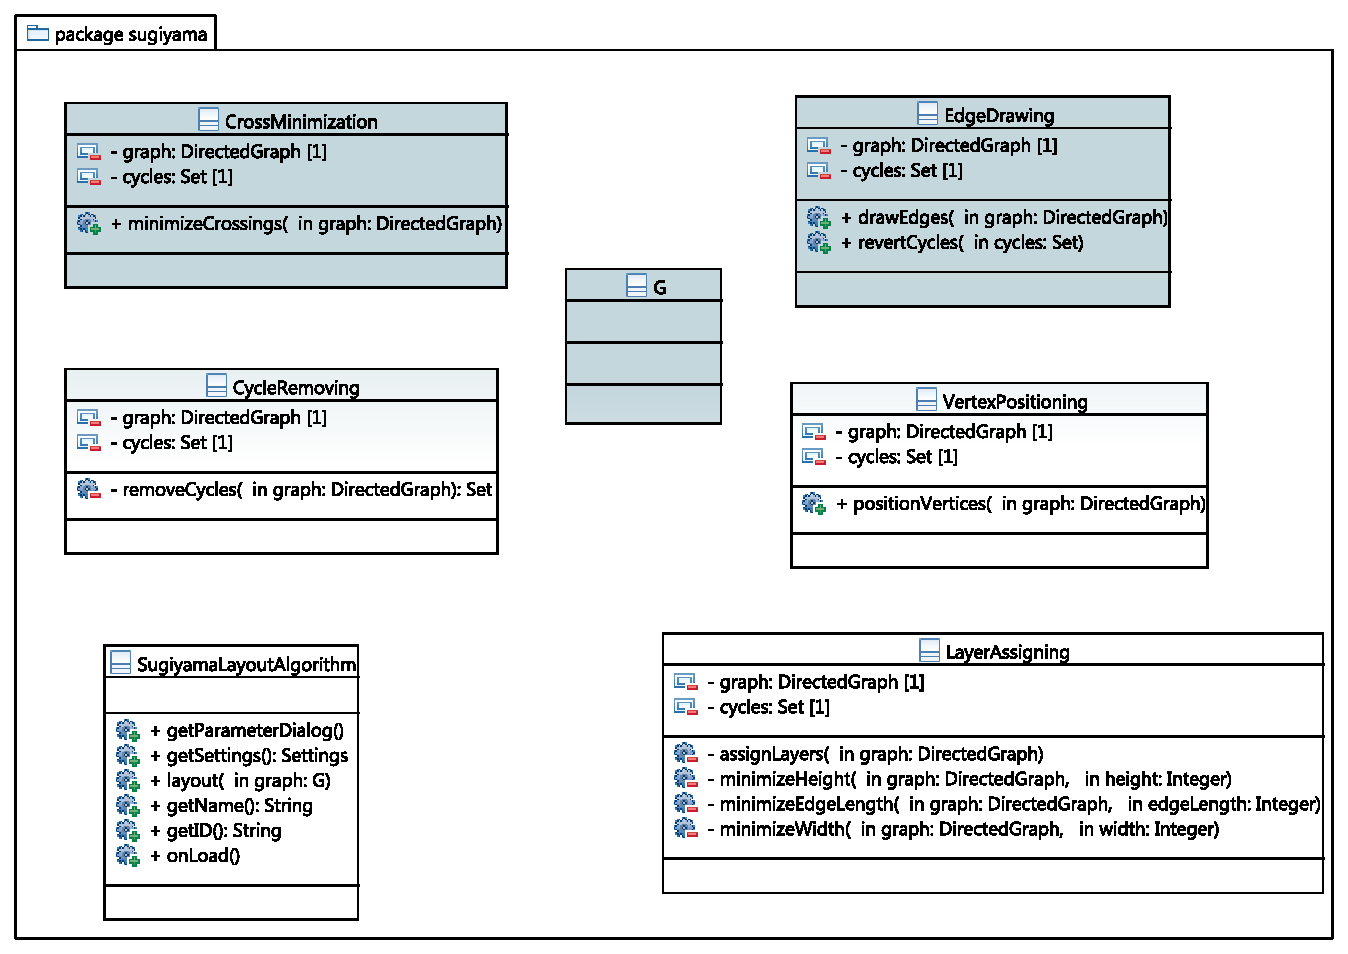
\includegraphics[width=380pt]{resourcen/sugiyama.pdf}
  \caption{Paketübersicht sugiyama}
  \label{fig:packge_sugiyama}
\end{figure}

Das Paket sugiyama bietet eine einfache Implementierung des Sugiyamaframeworks mit der bereits Graphen gelayoutet werden können. Es handelt sich hierbei um ein mitgeliefertes Plugin.

\newpage

\section{joana}

\begin{figure}[hb]
  \centering
  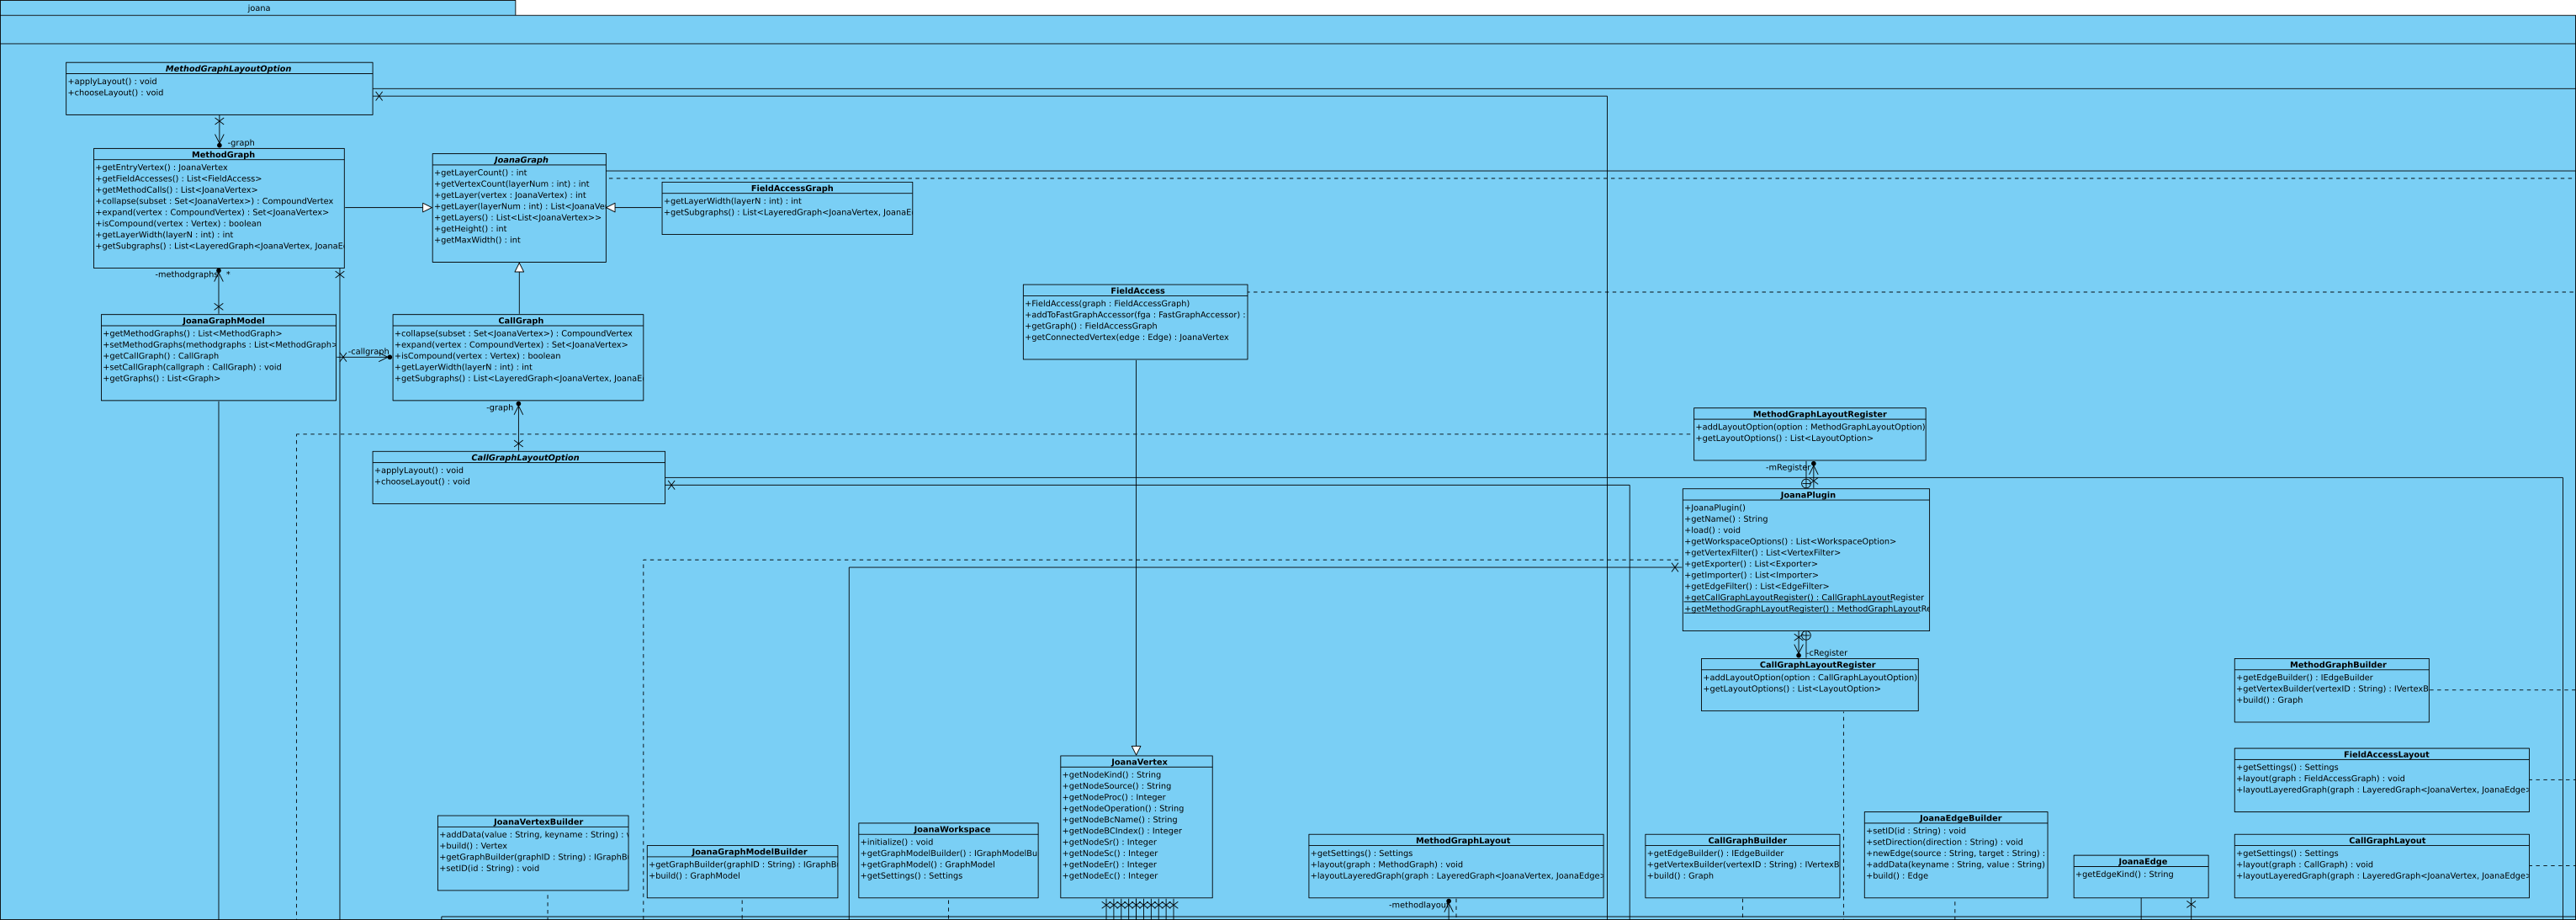
\includegraphics[width=380pt]{resourcen/joana.pdf}
  \caption{Paketübersicht joana}
  \label{fig:packge_joana}
\end{figure}

Das Paket Joana stellt ein weiteres mitgeliefertes Plugin dar und erweitert den sugiyama Algorithmus um spezifische Einstellungen und Constraints für Joana Graphen. Zu dem stellt es die Graphtypen Methoden- und Callgraph bereit, welche Joana spezifisch sind.